\documentclass[letterpaper]{article}
\usepackage[submission]{aaai2027}
\usepackage[hyphens]{url}
\usepackage{graphicx}
\urlstyle{rm}
\def\UrlFont{\rm}
\usepackage{natbib}
\usepackage{caption}
\usepackage{amsmath}
\usepackage{amssymb}
\usepackage{algorithm}
\usepackage{algorithmic}
\usepackage{booktabs}
\frenchspacing

\pdfinfo{/TemplateVersion (2027.1)}
\setcounter{secnumdepth}{0}
\newcommand{\method}{\textsc{DAFR}}

\title{From Policy Semantics to Safe Tool Execution: Semantic Lifting and Joint-Risk Certificates}
\author{Anonymous Submission}
\affiliations{}

\begin{document}
\maketitle
\noindent\textbf{Working revision:} The retained full AgentDojo and ASB tables are results of the original deterministic DAFR configuration, not the LLM-mapped extension. The mapper and matched geometry studies are reported as separate, frozen evidence because they answer semantic-transfer and execution-interface questions.

\noindent\textbf{Protocol-audit status:} The corrected mapper runner withholds hand-written labels, validates role semantics, and checks backend compilation. On a frozen 24-case cross-schema/paraphrase split, Qwen-Max produced 21/22 exact mappings on non-ambiguous cases and correctly abstained on 2/2 ambiguous cases; the matched schema-aware rules baseline produced 1/22 exact and 2/2 abstentions under the same IR/compiler/scorer. These mapper numbers are semantic-transfer evidence, not a replacement for the original full benchmark. On the same `src/clafr` runtime, a 512-case joint-risk suite found 25/512 false allows for independent axis thresholds, while Geometry and its equivalent predicate agreed on 512/512 decisions. In a 256-case executable repair suite, Geometry and Predicate+oracle each recovered 192 actions, while a bool-only predicate recovered none. We therefore claim a unified diagnostic/repair interface, not a security or expressiveness advantage over arbitrary if--else code.

\noindent Subsequent disjoint role-transfer probes use new tool names and preserve raw artifacts. The earlier v7--v11 splits are retained as development evidence; the v12 split is the primary cross-schema comparison because it includes paraphrased approval/confirmation language and renamed fields. All mapper artifacts retain raw responses, canonicalized IR, compiler status, and per-case scores.


\begin{abstract}
A tool call can be valid and relevant to the task yet still be induced by untrusted content and cause an unauthorized external effect. Execution therefore requires evidence that grounds the proposed effect, establishes its authorization, and matches the current state. We present DAFR, a policy-to-execution framework that performs semantic lifting from tool-specific schemas to a typed, auditable execution interface. A language-model mapper proposes the role and precondition map, while deterministic validation and compilation reject unsupported or ambiguous mappings. The resulting action--evidence point is evaluated against state-conditioned halfspaces and joint-risk regions, yielding an execution certificate with signed margins, provenance, and relation-specific feedback. Calls inside the feasible region are executed; calls outside it are blocked, clarified, or repaired when an admissible revision exists. On AgentDojo, DAFR reaches 0\% observed attack success with 87.5\% clean utility and 81.4\% attack utility. On Agent Security Benchmark, it reaches 0\% observed attack success with 86.8\% utility and 73.5\% task success. A held-out cross-schema study shows 21/22 exact non-ambiguous mappings for Qwen-Max versus 1/22 for a matched schema-aware rule mapper, while a joint-risk suite exposes 25 false allows by independent axis checks. These results connect semantic transfer to auditable tool execution without treating an arbitrary geometric implementation as intrinsically safer than equivalent predicate code.
\end{abstract}

\section{Introduction}

Tool-using agents can read private information, modify shared resources, contact external parties, and trigger actions that are difficult to reverse. These calls have more direct consequences than generated text: an executed call may immediately disclose information, change system state, or start an external operation \citep{yao2023react,schick2023toolformer,ruan2024toolemu,ye2024toolsword,lee2026mobilesafetybench}. Safe execution requires more than a valid schema. The function, effect-bearing arguments, expected effect, and state dependencies must be supported by the current task, available evidence, authorization, and policy.

Indirect prompt injection makes this decision difficult \citep{greshake2023indirectpromptinjection,liu2023promptinjection,zhan2024injecagent}. An agent may need untrusted content to complete a valid task, yet that content can contain attacker-inserted instructions. The model can translate them into a well-formed, apparently relevant call that discloses sensitive information, modifies the wrong object, or creates an unauthorized external effect \citep{NEURIPS2024_97091a51,liao2025eia,wang2025agentvigil,li2026agentdynagentsecuritydefenses,ma2026autodojoadaptiveblackboxattacks}. Tool descriptions and environment metadata provide additional channels for malicious control \citep{wang2026mcptox}. The execution-time question is whether trusted evidence supports the call's effect in the current state.

Consider an agent asked to update a customer record whose identifier is initially unknown. The agent retrieves the record, obtains its identifier from the verified result, and uses that identifier for the requested update. The retrieved content may also contain an attacker-issued command to send the record to a newly specified address. Both actions are schema-valid, but their support differs. The update follows the user request and uses an identifier established by the verified retrieval. The disclosure relies on a destination introduced through untrusted content and produces an unauthorized external effect. The execution layer must distinguish these actions by the evidence supporting their concrete effects.

Existing defenses act at different stages of the agent pipeline. Context-level methods separate trusted instructions from untrusted data, restructure prompts, repeat the user request, or filter suspicious observations before action generation \citep{hines2024spotlighting,wallace2024instructionhierarchy,jia2025taskshield,chen2025struq}. Runtime methods apply symbolic policies, privilege checks, execution plans, or information-flow rules to the generated action \citep{wang2025agentspec,shi2025progent,NEURIPS2025_77f3b26c,debenedetti2025defeatingpromptinjectionsdesign}. Tool-action feasibility, however, often depends on relations among the action, its evidence, and the current state. A destination can be valid when specified by the user and invalid when copied from a web page. A write can become feasible after a verified read establishes its target. Combining sensitive data with an external destination can require stronger grounding and authorization than either factor alone.

We introduce \method{} (Dynamic Action Feasible Regions), a policy-to-execution framework for deciding whether a concrete tool action is feasible at the current execution step. A semantic mapper first aligns tool-specific fields and policy requirements to a shared typed interface; deterministic validation, abstention, and compilation make this transfer auditable. The lifting function then represents the call and its supporting evidence as interpretable action--evidence coordinates. Policy-specified halfspaces and joint-risk regions encode the execution requirements active in the current state. Their intersection is an execution certificate: a call executes inside the region, and a call outside it is blocked or returned with feedback identifying the unsupported relation.

The certificate changes with execution. A verified read can establish an identifier required by a later write; a trusted confirmation can authorize a specific external effect; and a new observation can revise an earlier state assumption. DAFR reconstructs the action--evidence point and active constraints before every external effect. The mapper produces shared execution roles for tools with different schemas but comparable effects, and the same decision procedure then applies across tools. The mapper is used without parameter updates in our experiments, but the central contribution is the auditable semantic interface and its execution certificate rather than a claim that language-model mapping is universally training-free.

We evaluate DAFR on AgentDojo with three planner models and on Agent Security Benchmark (ASB) with DeepSeek V4 Flash. DAFR reaches 0\% observed attack success on both benchmarks, with 87.5\% clean utility and 81.4\% attack utility on AgentDojo and 86.8\% utility and 73.5\% task success on ASB. Removing geometric constraints raises attack success from 0\% to 16.7\%, and signed-margin analysis links each rejected call to the execution relation that limits feasibility. The consistent results across planners and benchmarks support DAFR as a unified execution-layer mechanism for reliable tool use. The evaluation protocol separately measures held-out-tool semantic transfer, so mapper generalization is not conflated with execution-layer security.

\begin{figure*}[t]
\centering
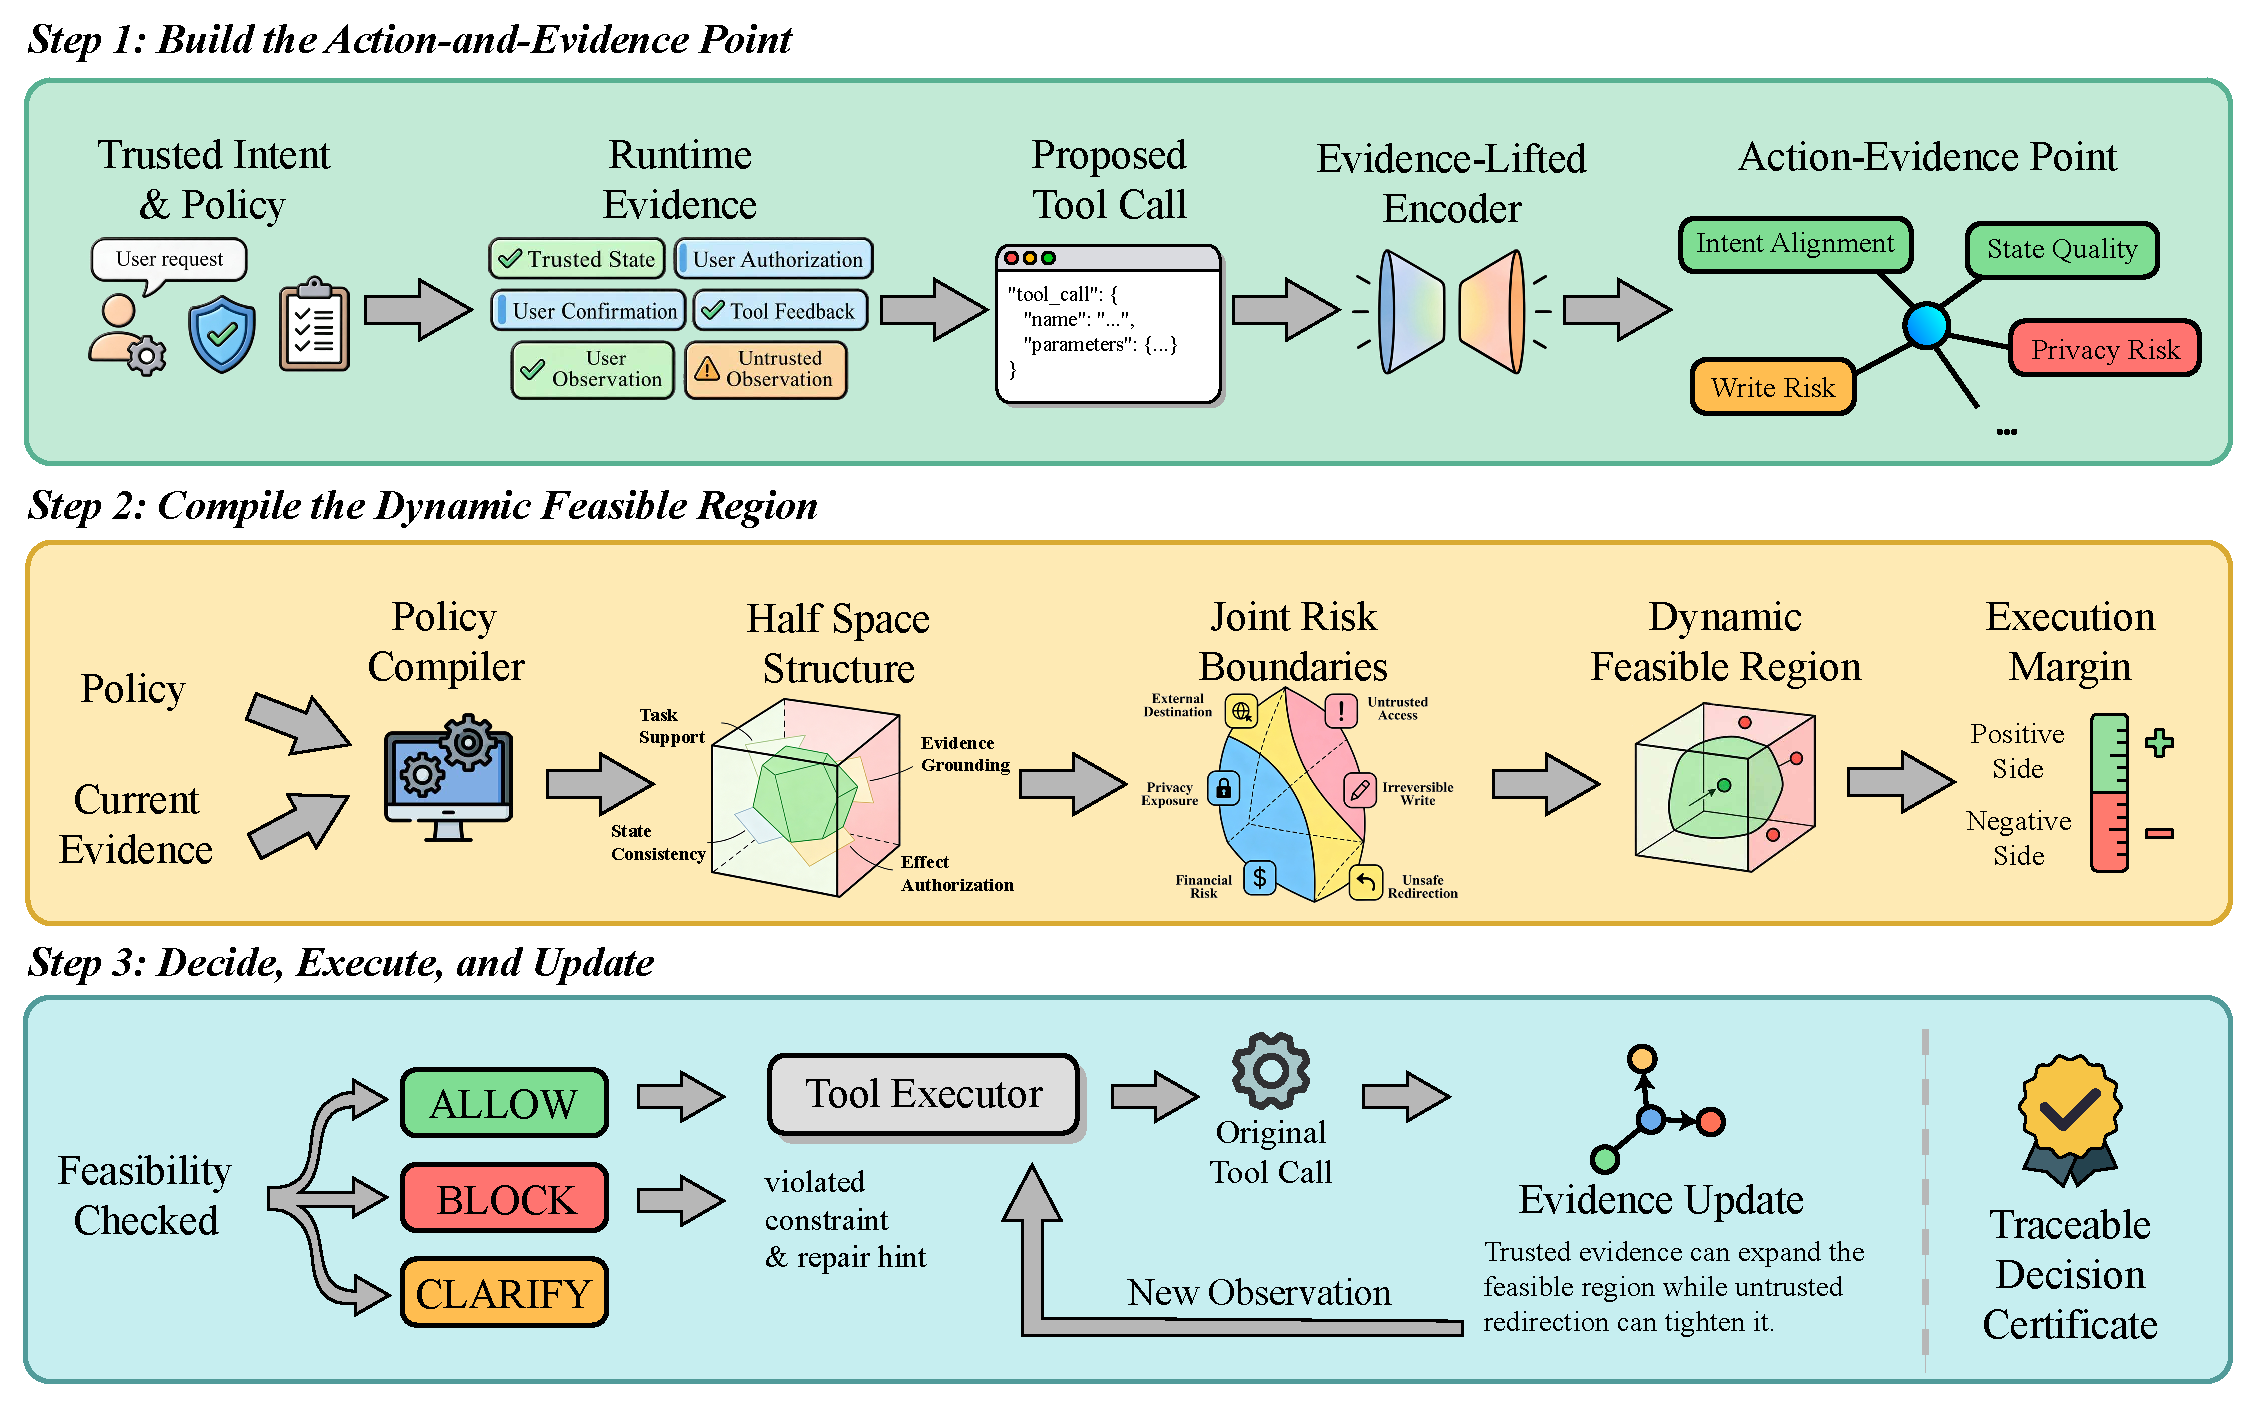
\includegraphics[width=\textwidth]{From_Semantics_to_Execution_Dynamic_Geometric_Constraints_for_Tool-Action_Feasibility_Figure_1.pdf}
\caption{Overview of DAFR. A proposed tool call and its runtime evidence define an action--evidence point. State-conditioned halfspaces and joint-risk boundaries form the current feasible region. Region membership determines feasibility, while violated margins identify the limiting relations used for targeted revision or blocking. The resulting observation updates the next decision state.}
\label{fig:mechanism}
\end{figure*}

\section{DAFR: Dynamic Action Feasible Regions}

DAFR constructs an interpretable action--evidence point for the proposed call and instantiates the geometric constraints active in the current state. Region membership determines feasibility, and signed margins identify the relations that limit the decision.

\subsection{Problem Setup}

At step $t$, a tool-using agent receives a trusted user task $u$, operates under an execution policy $p$, observes the environment, and produces a concrete tool call
\begin{equation}
 a_t=(f_t,\rho_t),
 \label{eq:tool-call}
\end{equation}
where $f_t$ is a registered tool and $\rho_t$ maps the fields of the tool schema to argument values. The call is first checked against the schema. Passing this check establishes that the call is well formed and leaves its execution feasibility to the evidence and policy checks below.

Let $E_t$ denote the execution state before $a_t$ is evaluated. It contains the trusted task, execution policy, available tool schemas, established facts, completed prerequisites, authorizations, confirmations, and observations with source labels. Facts derived from external observations retain their source labels, while intent, confirmation, and authorization are recorded through trusted channels.

A call is feasible when the current evidence and policy support its function, the arguments that determine its external effect, the expected effect itself, and the required state conditions. We write
\begin{equation}
 \operatorname{Feas}(a_t\mid E_t,u,p)=1
 \label{eq:feasibility}
\end{equation}
when these conditions are satisfied. A feasible call is sent to the trusted runtime. An infeasible call is blocked or returned with feedback that identifies the function, argument, evidence source, authorization condition, or state assumption requiring revision. After an admitted call returns observation $o_{t+1}$, the state is updated as
\begin{equation}
 E_{t+1}=T(E_t,a_t,o_{t+1}),
 \label{eq:state-transition}
\end{equation}
where $T$ may add evidence, satisfy a prerequisite, record authorization, or invalidate an earlier assumption.

\subsection{Action--Evidence Point Construction}

DAFR represents each proposed tool call and its current evidence as a point in an interpretable action--evidence space. The coordinates cover task support and progress, argument grounding and provenance, authorization and scope, and expected effects and risks.

DAFR uses a semantic mapper followed by deterministic validation and a semantic lifting function to construct the action--evidence point:
\begin{equation}
 z_t=L(a_t,E_t,u,p)=(q_t,g_t,c_t,r_t)\in[0,1]^d,
 \label{eq:action-evidence-point}
\end{equation}
where $L$ deterministically evaluates explicit execution relations after the mapper has produced a validated typed interface, and $q_t$, $g_t$, $c_t$, and $r_t$ are the resulting coordinate blocks. The task block $q_t$ records support for the selected function, its expected effect, and current execution progress. The grounding block $g_t$ connects effect-bearing arguments to source-tagged evidence and established state. The authorization block $c_t$ records confirmation, available authority, and the scope of the proposed effect. The risk block $r_t$ describes consequences such as disclosure, transfer, deletion, redirection, and state change.

The mapper receives the trusted policy text and the registered schema and returns a typed constraint intermediate representation (IR). The IR records field roles, trusted preconditions, authorization requirements, and risk budgets. Structural validation rejects unknown fields, unsupported roles, non-trusted authorization sources, and out-of-range budgets. A canonicalizer corrects only high-confidence role slips using trusted field descriptions; unresolved ambiguity produces abstention. Validation is not a semantic oracle: mapper omission and mistranslation are measured separately, and failed validation is handled conservatively.

For each tool $f$, a role map
\begin{equation}
 B_f:\operatorname{Fields}(f)\rightarrow\mathcal U
 \label{eq:role-map}
\end{equation}
maps tool-specific fields to execution roles in $\mathcal U$, including destination, object, data, amount, time, and effect. In our no-parameter-update setting, $B_f$ is supplied by the validated mapper output rather than a hand-written per-tool table. Recipients, payment accounts, and sharing targets map to the destination role; records, files, messages, and transaction details map to data or object roles; and reads, writes, disclosures, transfers, and deletions map to effect roles. The original field and value are retained so that feedback can name the exact argument that requires revision.

The encoder consumes the validated role map before applying legacy name heuristics. In particular, a mapped destination such as an owner or assignee contributes to external-sink risk even when its field name does not contain recipient-like tokens; this keeps semantic transfer and feature extraction on the same typed interface.

The evidence used by these relations is maintained in the execution state. After an admitted call returns $o_{t+1}$, an evidence projection operator converts it into source-tagged factual and risk records:
\begin{equation}
 P(o_{t+1})=\left(S_{t+1}^{+},R_{t+1}^{+}\right),
 \label{eq:evidence-projection}
\end{equation}
where $S_{t+1}^{+}$ contains entities, argument values, completed prerequisites, and observed state changes, and $R_{t+1}^{+}$ contains untrusted instructions, task conflicts, unsupported effect requests, and other risk signals. Each record retains its source, trust status, and execution role when incorporated into $E_{t+1}$. Factual records update grounding and state relations, risk records update source, conflict, and effect-risk relations, and trusted records establish intent, confirmation, and authorization.

Each coordinate has a defined execution meaning and takes a value in $[0,1]$ under the current call and execution state. Coordinates for prerequisites and authorization record whether the corresponding conditions have been established, while grounding and scope coordinates record the support available for a specific argument or effect from source-tagged evidence. For example, a verified lookup can establish the identifier required by a later update, whereas a destination introduced by untrusted content receives no authorization support for an external disclosure.

For an effectful call, let $V(a_t)$ denote the argument values that directly determine its external effect, such as a destination, object identifier, amount, date, or sensitive data. DAFR evaluates each value against the trusted task, source-tagged evidence, and current state. The critical grounding score is
\begin{equation}
 g_{\mathrm{crit}}(a_t,E_t)=\min_{v\in V(a_t)} g(v,E_t),
 \label{eq:critical-grounding}
\end{equation}
where $g(v,E_t)\in[0,1]$ measures the available support for value $v$. The minimum gives a conjunctive grounding summary across the arguments that determine the external effect: every critical value must satisfy its grounding requirement. Schema-optional fields follow the same effect-aware check. A field is eligible for omission during revision only when its removal leaves the destination, object, data, scope, authorization requirements, and expected external effect unchanged. Otherwise, an unsupported value keeps the call infeasible.

As evidence and execution state evolve, DAFR updates the affected coordinates, so the same proposed call may occupy a different position at a later execution step.

\subsection{Dynamic Geometric Constraints}

DAFR converts the execution requirements at step $t$ into geometric regions in the action--evidence space. Each policy is compiled from the validated IR into constraint templates and coefficients before evaluation. The runtime parameters are frozen after compilation and are not tuned on the evaluated trajectory. For a proposed call, its expected effect, available evidence, authorization scope, policy, and current state select the active templates. Let $\mathcal H_t=\mathcal H(a_t,E_t,u,p)$ denote requirements expressed through individual execution relations. Each $j\in\mathcal H_t$ defines a halfspace
\begin{equation}
 \mathcal P_j=\left\{z\in[0,1]^d\mid m_j^{\mathrm{half}}(z)=b_j-w_j^\top z\geq0\right\}.
 \label{eq:halfspace}
\end{equation}
For each active requirement, the policy compiler retrieves $w_j$ and $b_j$ from the corresponding fixed template. The vector $w_j$ selects and weights the relevant execution relations, and $b_j$ sets the feasibility boundary. The coefficient signs follow the semantic direction of each relation: stronger trusted support raises the margin, and greater execution risk lowers it. These halfspaces represent task support, completed prerequisites, state consistency, critical-argument grounding, destination validity, confirmation, and authorization.

Some conditions depend on several relations at once. Let $\mathcal K_t=\mathcal K(a_t,E_t,u,p)$ denote the joint-risk conditions active at step $t$. Each $k\in\mathcal K_t$ defines a joint margin and its feasible region:
\begin{equation}
\begin{aligned}
 m_k^{\mathrm{joint}}(z)&=\beta_k+v_k^\top C_kz-\lVert W_kR_kz\rVert_2,\\
 \mathcal C_k&=\left\{z\in[0,1]^d\mid m_k^{\mathrm{joint}}(z)\geq0\right\}.
\end{aligned}
 \label{eq:joint-region}
\end{equation}
The template for risk family $k$ specifies the selectors $C_k$ and $R_k$, the support weights $v_k$, the risk weights $W_k$, and the base risk budget $\beta_k$. The selectors extract the support and risk coordinates used by the condition. The support and risk weights are nonnegative, preserving the semantic direction of the joint margin. The curved boundary makes the acceptable level of each risk depend on the other risks present and the trusted support available for the action.

The feasible region is the intersection of all applicable regions:
\begin{equation}
 \mathcal F_t=\left(\bigcap_{j\in\mathcal H_t}\mathcal P_j\right)\cap\left(\bigcap_{k\in\mathcal K_t}\mathcal C_k\right).
 \label{eq:feasible-region}
\end{equation}
Only points that satisfy every relevant requirement belong to $\mathcal F_t$. DAFR instantiates this geometry at every step through the current $z_t$, $\mathcal H_t$, and $\mathcal K_t$. New evidence can move the point, introduce relevant boundaries, or satisfy conditions that previously prevented execution.

The running example shows how this geometry changes over a trajectory. Before the lookup returns, the update lacks the record identifier required by its grounding and prerequisite relations. The verified lookup establishes that value and allows the update point to enter the feasible region. The same observation provides no authority for an unrelated disclosure. That action combines an untrusted destination, sensitive data, and an external effect without matching authorization, so it remains outside $\mathcal F_t$. Evidence can therefore support one concrete effect while leaving another infeasible because the calls depend on different roles, sources, and authorization conditions.

\subsection{Geometric Properties}

\paragraph{Convexity and semantic direction.}
For a fixed execution context, every $\mathcal P_j$ is a halfspace. Each joint margin in Eq.~\eqref{eq:joint-region} is concave because it is an affine function minus a norm, so its superlevel set $\mathcal C_k$ is convex. Their intersection $\mathcal F_t$ is therefore convex and defines one coherent feasible region for the current decision.

The parameter signs preserve a common semantic direction across the geometry. Trusted grounding, confirmation, and authorization increase the relevant margins, while externality, sensitivity, irreversibility, and untrusted control decrease them. Support and risk therefore move an action toward opposite sides of the active boundaries.

\paragraph{Joint risks.}
The curved regions capture how the acceptable level of one risk changes with the other risks present and with the trusted support available for the action. When multiple risk relations share one authorization budget, the norm term in Eq.~\eqref{eq:joint-region} permits different allocations while limiting their combined magnitude. An increase in one risk reduces the amount of the others that can be accepted under the same evidence and authorization.

\paragraph{Source-aware state changes.}
New records update the relations they establish. A verified read can increase grounding and prerequisite support for returned values; a trusted confirmation can increase scoped authorization for a specified effect, object, or destination; and an untrusted observation can contribute factual values while activating source, conflict, or redirection risks. These source-aware updates allow one observation to support a requested write while leaving an unrelated disclosure outside the feasible region.

\subsection{Feasibility Decision and Targeted Feedback}

Given $z_t$, DAFR evaluates every margin that defines $\mathcal F_t$. The overall feasibility margin is
\begin{equation}
 M_t(z)=\min\left\{\min_{j\in\mathcal H_t}m_j^{\mathrm{half}}(z),\;\min_{k\in\mathcal K_t}m_k^{\mathrm{joint}}(z)\right\}.
 \label{eq:overall-margin}
\end{equation}
Because membership in $\mathcal F_t$ requires every active margin to be nonnegative,
\begin{equation}
 z_t\in\mathcal F_t\quad\Longleftrightarrow\quad M_t(z_t)\geq0.
 \label{eq:membership}
\end{equation}
The sign of $M_t(z_t)$ is equivalent to region membership, and its magnitude records the raw signed slack under the most limiting active condition. DAFR executes the call when $M_t(z_t)\geq0$. When an admissible revision path exists, a failed condition produces targeted feedback for the planner. All other infeasible calls are blocked.

A call may violate several boundaries. DAFR records
\begin{equation}
 \mathcal V_t=\left\{c\in\mathcal H_t\cup\mathcal K_t\mid m_c(z_t)<0\right\},
 \label{eq:violated-set}
\end{equation}
where $m_c$ denotes the halfspace or joint margin associated with condition $c$. For feedback ordering, DAFR places violated margins on comparable scales through $\overline m_c(z_t)=m_c(z_t)/\sigma_c$, with $\sigma_c>0$. Raw margins continue to determine feasibility. The most limiting conditions are selected from $\mathcal V_t$, and $\phi_t=\Gamma(\mathcal V_t,z_t,E_t)$ maps them to concise revision targets. Feedback can identify an unsupported tool choice or argument, an unsuitable source, missing authorization, an incomplete prerequisite, an outdated state assumption, or the factors contributing to a joint-risk violation.

Each decision records the concrete call, its action--evidence point, the active boundaries, the margin vector, and the supporting evidence links. This record provides the same geometric basis for the execution decision and the revision target.

\begin{algorithm}[tb]
\caption{DAFR Execution-Step Decision}
\label{alg:dafr-step}
{\raggedright
\textbf{Input}: proposed call $a_t=(f_t,\rho_t)$, state $E_t$, task $u$, policy $p$.\par
\textbf{Output}: execution decision and feedback.\par
}
\begin{algorithmic}[1]
\STATE Check $a_t$ against the registered schema of $f_t$.
\STATE Map tool fields to shared execution roles with $B_{f_t}$.
\STATE Build $z_t=L(a_t,E_t,u,p)$ from the current relations.
\STATE Instantiate $\mathcal H_t$ and $\mathcal K_t$ from the active policy templates.
\STATE Evaluate all active margins and compute $M_t(z_t)$.
\IF{$M_t(z_t)\geq0$}
\STATE Execute $a_t$, obtain $o_{t+1}$, and update $E_{t+1}$.
\ELSE
\STATE Form $\mathcal V_t$ and derive feedback $\phi_t$.
\IF{an admissible revision path exists}
\STATE Return \textsc{Clarify} with $\phi_t$ to the planner.
\ELSE
\STATE Return \textsc{Block}.
\ENDIF
\ENDIF
\end{algorithmic}
\end{algorithm}

\subsection{Runtime Update and Cost}

Each invocation of DAFR evaluates one concrete proposed call. A feasible call is executed by the trusted runtime, and the returned observation is projected into source-tagged records and incorporated into the next execution state through Eqs.~\eqref{eq:evidence-projection} and~\eqref{eq:state-transition}. An infeasible call produces no external effect. When targeted feedback is returned, the planner may revise the call, obtain additional evidence, request authorization, or end the task. Any subsequent proposal is evaluated as a new call under the state available at that step.

\paragraph{Runtime cost and local updates.}
Let $C_t=|\mathcal H_t|+|\mathcal K_t|$ denote the number of geometric regions evaluated at step $t$, and let $s_c$ denote the number of coordinates used by region $c$. Computing the complete margin vector requires
\begin{equation}
 O\left(\sum_{c=1}^{C_t}s_c\right)\leq O(C_td)
 \label{eq:runtime-cost}
\end{equation}
operations. Each region uses only a subset of the execution relations, so margin evaluation scales with the active regions and the coordinates they select.

Observations from admitted tool executions or trusted user interactions update only the relations linked to the affected values, sources, authorization conditions, and state facts. Before evaluating the next proposed external effect, DAFR constructs its action--evidence point and reevaluates every applicable margin. Local relation updates and complete margin reevaluation limit computation to the active regions and their selected coordinates while preserving a full feasibility check for each proposal.

\section{Evaluation}

\subsection{Experimental Setup}

AgentDojo v1.2.2 is the primary benchmark and contains the Banking, Slack, Travel, and Workspace suites \citep{NEURIPS2024_97091a51}. We evaluate DeepSeek V4 Flash, GPT-5.4-mini, and Claude Haiku 4.5 on the same 71 clean and 585 attacked cases for each planner. The comparison includes DAFR and eight baselines. Figure~\ref{fig:agentdojo-main} presents six representative methods, and the supplement reports the complete results. Component ablations evaluate evidence projection, action--evidence lifting, geometric constraints, and decision feedback.

We further evaluate DAFR on 204 ASB cases using DeepSeek V4 Flash \citep{zhang2025agentsecuritybench}. AgentDojo reports clean utility, attack utility, and attack success rate (ASR), while ASB reports utility, task success, and ASR.

DAFR is placed at the execution boundary, after the planner proposes a concrete tool call and before the trusted runtime performs its external effect. Each comparison keeps the benchmark cases, planner model, registered tools, and tool schemas fixed. Under this setup, DAFR contributes the feasibility decision and relation-specific revision feedback for the proposed call, while the benchmark task and planning environment remain unchanged. The mapper is evaluated on a disjoint held-out tool split and is frozen before end-to-end evaluation.
\paragraph{Mapper and representation protocol.}
The mapper is evaluated before end-to-end execution on a disjoint held-out tool split. We report role accuracy, prerequisite recall, omitted-policy rate, unsafe relaxation rate, abstention, latency, and token cost. A mapping that fails structural validation is rejected and is not counted as successful transfer. For the geometry ablation, Boolean predicates, axis-aligned thresholds, weighted halfspaces, and joint-risk cones share the same validated IR, semantic features, evidence state, candidate actions, and repair candidates. The unrestricted predicate control is an implementation-equivalent decision check; therefore any difference in the accept/reject bit is treated as a bug. The comparison targets the restricted axis-threshold baseline, margin-based diagnostics, repair quality, and execution cost.

As the primary mapper comparison, the frozen v12 split contains 24 tools absent from the few-shot examples and includes renamed fields plus approval/confirmation paraphrases. Qwen-Max produced 22 compilable candidates and 21/22 exact non-ambiguous mappings, while the matched schema-aware rules control produced 14 compilable candidates and 1/22 exact. Both methods abstained on the two ambiguous policies. These numbers measure semantic transfer after validation, not end-to-end attack success; the full AgentDojo and ASB tables therefore remain separate.

As a task-level transfer check, we froze the same Qwen-Max planner, Banking tasks, CLAFR runtime, and 16-clean/144-attack denominator while changing only the mapper execution mode. The strict IR mode obtained 8/16 clean and 73/144 attack utility; a matched no-mapper runtime obtained 9/16 and 71/144; and \emph{roles-only} semantic lifting, which retains validated roles but leaves the final envelope to the deterministic runtime, obtained 10/16 and 77/144. All three configurations had 0/144 observed ASR. This is a Banking-only extension rather than a replacement for the full deterministic multi-suite table, but it shows why the mapper should provide a typed semantic interface instead of duplicating hard execution gates.

\begin{table}[ht]
\centering
\small
\setlength{\tabcolsep}{3.5pt}
\begin{tabular}{lrrrr}
\toprule
Mapper & Compilable & Exact/22 & Abstain/2 & Unsafe relax.\\
\midrule
Schema-aware rules & 14 & 1 & 2 & 11\\
Qwen-Max + validator & 22 & 21 & 2 & 1\\
\bottomrule
\end{tabular}
\caption{Held-out cross-schema mapper comparison. Exact scores use the 22 non-ambiguous cases; the two ambiguous policies are scored separately for correct abstention.}
\label{tab:mapper-transfer}
\end{table}

\begin{figure*}[t]
\centering
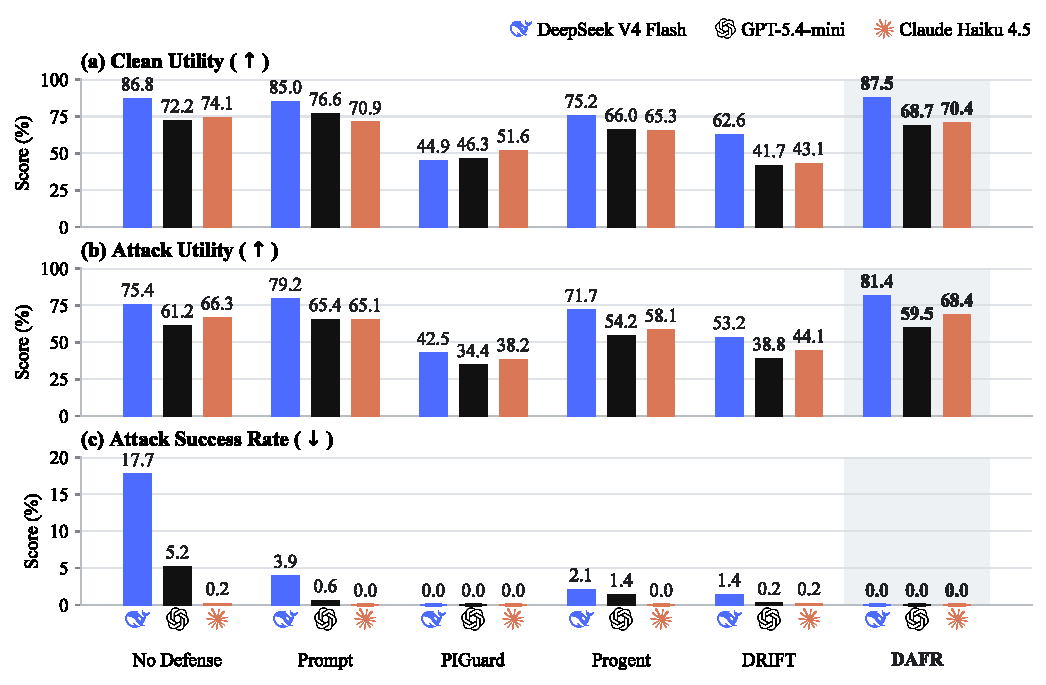
\includegraphics[width=\textwidth]{From_Semantics_to_Execution_Dynamic_Geometric_Constraints_for_Tool-Action_Feasibility_Figure_2.pdf}
\caption{AgentDojo clean utility, attack utility, and attack success rate across six representative methods and three planner models. Values are percentages; arrows indicate the preferred direction. The supplement reports all nine evaluated methods.}
\label{fig:agentdojo-main}
\end{figure*}

\subsection{Main Results on AgentDojo}

Figure~\ref{fig:agentdojo-main} reports the AgentDojo comparison across three planner models. With DeepSeek V4 Flash, DAFR achieves 87.5\% clean utility and 81.4\% attack utility with 0\% observed ASR. DAFR also records 0\% observed ASR with GPT-5.4-mini and Claude Haiku 4.5, while retaining 59.5\% and 68.4\% attack utility, respectively.

PIGuard is the only other representative method that reaches 0\% observed ASR with all three planners. At this security level, DAFR improves attack utility over PIGuard by 38.9, 25.1, and 30.2 percentage points on DeepSeek, GPT, and Claude, respectively. The feasible-region decision preserves more task progress under attack while maintaining zero observed attack success.

\subsection{Results on Agent Security Benchmark}

Table~\ref{tab:asb-main} reports results on 204 ASB cases with DeepSeek V4 Flash. DAFR achieves 86.8\% utility and 73.5\% task success with 0\% observed ASR.

\begin{table}[!ht]
\centering
\small
\setlength{\tabcolsep}{4pt}
\begin{tabular}{lrrr}
\toprule
Method & Utility & Task Succ. & ASR\\
\midrule
No Defense & 88.7 & 77.9 & 90.2\\
Delimiter & 87.3 & 77.0 & 86.3\\
Instruction Prevention & 88.0 & 77.5 & 39.7\\
Observation Sandwich & 88.0 & 77.0 & 27.9\\
TS-Flow & 85.5 & 73.5 & 19.1\\
Progent & 86.0 & 73.0 & 3.4\\
DRIFT & 85.8 & 73.0 & 23.0\\
\textbf{DAFR} & 86.8 & 73.5 & \textbf{0.0}\\
\bottomrule
\end{tabular}
\caption{Results on 204 ASB cases with DeepSeek V4 Flash. Values are percentages.}
\label{tab:asb-main}
\end{table}

Compared with no defense, DAFR reduces ASR from 90.2\% to 0\%, with a 1.9-point difference in utility. Among the evaluated methods, DAFR is the only one that reaches 0\% observed ASR. Relative to Progent, the strongest competing method by ASR, DAFR gains 0.8 points in utility and 0.5 points in task success and reduces ASR from 3.4\% to 0\%. The ASB results extend DAFR's security--utility balance beyond AgentDojo to a distinct tool-use benchmark.

\subsection{Ablation and Geometric Analysis}

Table~\ref{tab:ablation} reports the full AgentDojo ablation with DeepSeek V4 Flash: each configuration uses the same 71 clean and 585 attacked cases across four suites, with suite-macro-averaged scores. Removing evidence projection lowers clean utility from 87.5\% to 79.2\% while retaining 81.8\% attack utility and 0\% observed ASR. Removing action--evidence lifting raises clean and attack utility to 91.5\% and 85.3\% but introduces a 0.7\% observed ASR.

Removing geometric constraints produces the largest security change in the original module ablation: observed ASR rises from 0\% to 16.7\%, with attack utility at 81.3\%. This module ablation also removes geometry-conditioned observation handling, so it does not isolate the syntax of geometry from the underlying policy checks. We therefore add a matched representation ablation: Boolean predicates, axis-aligned thresholds, weighted halfspaces, and joint-risk cones consume the same mapper output, features, evidence, and candidate actions. The general predicate and geometric implementations are expected to agree on membership; the scientific comparison concerns axis-threshold expressiveness, margin-based diagnosis, and executable repair, not a claim that geometry can express functions unavailable to unrestricted programs. In a frozen 512-case joint-risk suite, independent axis thresholds allowed all cases and falsely allowed 25 actions whose joint risk exceeded the shared budget; the joint cone and equivalent predicate both allowed 487/512 and disagreed on 0/512. In a matched 256-case action suite, Geometry and Predicate+oracle each recovered 192 executable actions, while a bool-only predicate recovered 0; all 64 non-repairable actions remained blocked. This is evidence about coupled-budget encoding and an auditable repair interface, not arbitrary-program superiority. Removing decision and feedback lowers clean and attack utility to 79.4\% and 80.0\% and introduces a 0.8\% observed ASR.

\begin{table}[ht]
\centering
\small
\setlength{\tabcolsep}{3.5pt}
\begin{tabular}{lrrr}
\toprule
Configuration & Clean & Attack & ASR\\
\midrule
DAFR & 87.5 & 81.4 & 0.0\\
w/o Evidence Projection & 79.2 & 81.8 & 0.0\\
w/o Action--Evidence Lifting & 91.5 & 85.3 & 0.7\\
w/o Geometric Constraints & 90.2 & 81.3 & 16.7\\
w/o Decision \& Feedback & 79.4 & 80.0 & 0.8\\
\bottomrule
\end{tabular}
\caption{Component ablation on AgentDojo. Values are percentages.}
\label{tab:ablation}
\end{table}
\paragraph{Signed-margin behavior.}
Table~\ref{tab:agentdojo-margin-summary} summarizes the overall signed margins of 9{,}083 AgentDojo tool calls across three planner models. Because DAFR admits a call exactly when $M_t(z_t)\geq0$, the analysis reports the magnitude of the raw signed slack produced by the active constraints. Mean margins are 0.712--0.750 for admitted calls and $-0.368$ to $-0.214$ for rejected calls. For each rejected call, the active condition attaining the minimum margin identifies the prerequisite, argument, source, authorization condition, or joint-risk relation used for targeted feedback.

\begin{table}[ht]
\centering
\small
\setlength{\tabcolsep}{4.5pt}
\begin{tabular}{lrrr}
\toprule
Planner & Calls & $\overline M_{\mathrm{adm}}$ & $\overline M_{\mathrm{rej}}$\\
\midrule
DeepSeek V4 Flash & 3947 & 0.712 & $-0.368$\\
GPT-5.4-mini & 2916 & 0.748 & $-0.214$\\
Claude Haiku 4.5 & 2220 & 0.750 & $-0.289$\\
\bottomrule
\end{tabular}
\caption{Mean signed margins for admitted and rejected AgentDojo calls.}
\label{tab:agentdojo-margin-summary}
\end{table}

\section{Related Work}

\paragraph{Prompt-injection attacks and defenses.}
Indirect prompt injection allows untrusted observations to redirect tool-using agents, as shown by early attacks and later benchmarks \citep{greshake2023indirectpromptinjection,liu2023promptinjection,zhan2024injecagent,NEURIPS2024_97091a51}. Context-level defenses preserve instruction boundaries, prioritize trusted instructions, or separate instructions from data \citep{hines2024spotlighting,wallace2024instructionhierarchy,chen2025struq}. PIGuard detects injected content, Task Shield checks task alignment, and MELON compares normal execution with masked re-execution \citep{li2025piguard,jia2025taskshield,zhu2025melon}.

\paragraph{Runtime controls for tool-using agents.}
AgentSpec and ShieldAgent express runtime requirements through explicit safety policies \citep{wang2025agentspec,chen2025shieldagent}. Progent enforces privileges over tool names and arguments, and DRIFT checks deviations from a task-grounded function trajectory \citep{shi2025progent,NEURIPS2025_77f3b26c}. CaMeL separates control and data flows derived from a trusted request, and Fides enforces confidentiality and integrity labels \citep{debenedetti2025defeatingpromptinjectionsdesign,costa2025fides}.

\paragraph{Tool-safety evaluation.}
ToolEmu and ToolSword study failures arising from consequential tool use \citep{ruan2024toolemu,ye2024toolsword}. AgentHarm and MobileSafetyBench extend evaluation to harmful multi-step behavior and mobile-device control, and MCPTox studies tool poisoning in MCP servers \citep{andriushchenko2025agentharm,lee2026mobilesafetybench,wang2026mcptox}. Our evaluation uses AgentDojo and ASB to measure task utility and attack-induced tool effects.

\paragraph{Geometric safety formulations.}
Action shielding restricts decisions to actions that satisfy formal safety specifications \citep{alshiekh2018shielding}. GIF uses model Jacobians and local output geometry to bound information flow inside language models \citep{storek2026gif}. DAFR instead places explicit action--evidence relations at the execution boundary. State-conditioned halfspaces and joint-risk regions combine task support, grounding, provenance, authorization, effects, and state in one feasibility decision, and active margins provide relation-specific revision targets.

\section{Limitations}

DAFR is evaluated on AgentDojo and ASB with three planner models, covering multiple tool suites, execution patterns, and risk categories. This scope establishes its behavior under two complementary benchmark protocols. Evaluation in additional domains can characterize its operation with other tools and execution settings.

DAFR derives support from tool outputs, environment observations, and trusted user interactions. If the required evidence, authorization, or state condition has not been established, the call remains outside the feasible region and DAFR requests the admissible support or blocks execution. Missing evidence is thus represented as an explicit execution state rather than treated as implicit approval.

New tools are mapped by the semantic mapper and deterministic validation stack. We report held-out-tool mapping accuracy, omitted requirements, unsafe relaxation rate, abstention, latency, and token cost before using a mapping in the end-to-end run. A mapper failure is not treated as successful generalization. A tool with a genuinely new behavior or control structure may still require a new role or policy template. The retained AgentDojo and ASB tables use the deterministic DAFR configuration; the mapper study is a separate semantic-transfer evaluation rather than a claim that mapper accuracy alone establishes benchmark-level security.

\section{Conclusion}

Tool calls can be well formed and relevant to a task yet lack the evidence, authorization, or state support required for execution. DAFR addresses this gap with policy-to-execution semantic lifting, a typed policy-to-IR interface, a deterministic action--evidence representation, and a dynamic feasible region formed by policy-specified halfspaces and joint-risk constraints. The mapper can operate without parameter updates in our experiments, while validation and abstention prevent uncertain mappings from silently becoming executable policy. The geometric representation is useful because it composes coupled risk budgets and exposes signed margins for diagnosis and repair; it is not claimed to be more expressive than unrestricted if--else code. Calls inside the region execute; calls outside it are blocked or returned with relation-specific feedback.

On AgentDojo and Agent Security Benchmark, DAFR reaches 0\% observed attack success while retaining task utility across tool environments and planner models. The matched ablation tests which benefits arise from the decision representation, while the signed margins connect rejected calls to their limiting execution relations. The central hypothesis is that a typed semantic interface plus a joint-risk execution certificate improves cross-schema transfer, compositional risk handling, and repair observability. Its accept/reject bit is intentionally matched to an equivalent predicate, so the contribution is the unified certificate, diagnostics, provenance, and runtime composition. Together, these results establish dynamic feasible regions as an execution-layer formulation that turns task evidence, authorization, and state into auditable tool-action decisions.

\bibliography{From_Semantics_to_Execution_Dynamic_Geometric_Constraints_for_Tool-Action_Feasibility_References}
\end{document}
